\begin{figure*}[t]
\centering
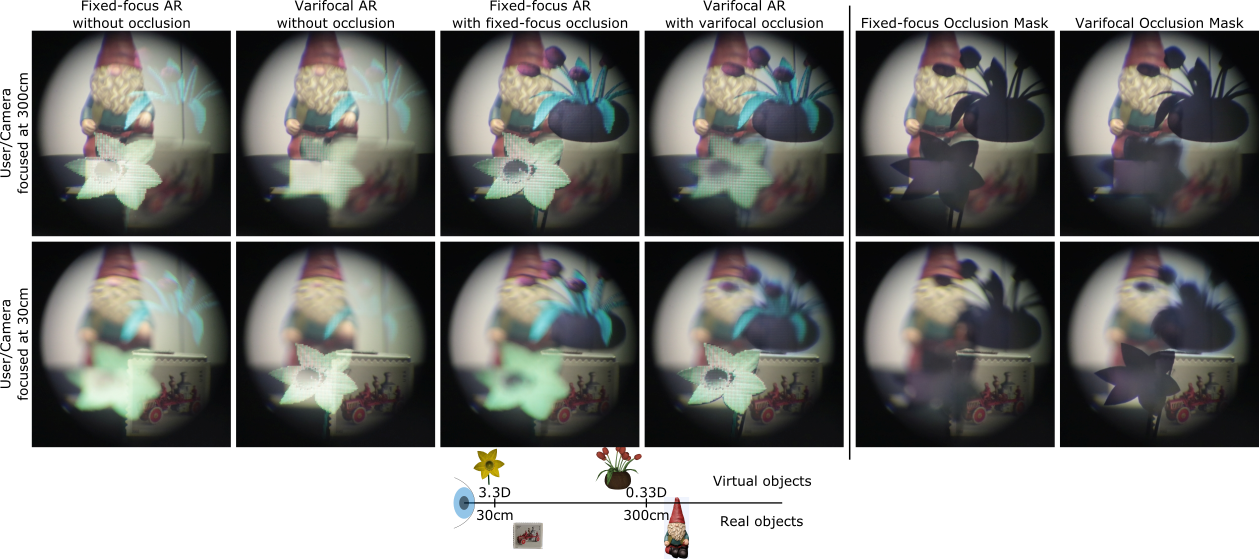
\includegraphics[width=0.99\textwidth]{images/varifocal_occlusion/teaser}
%\fbox{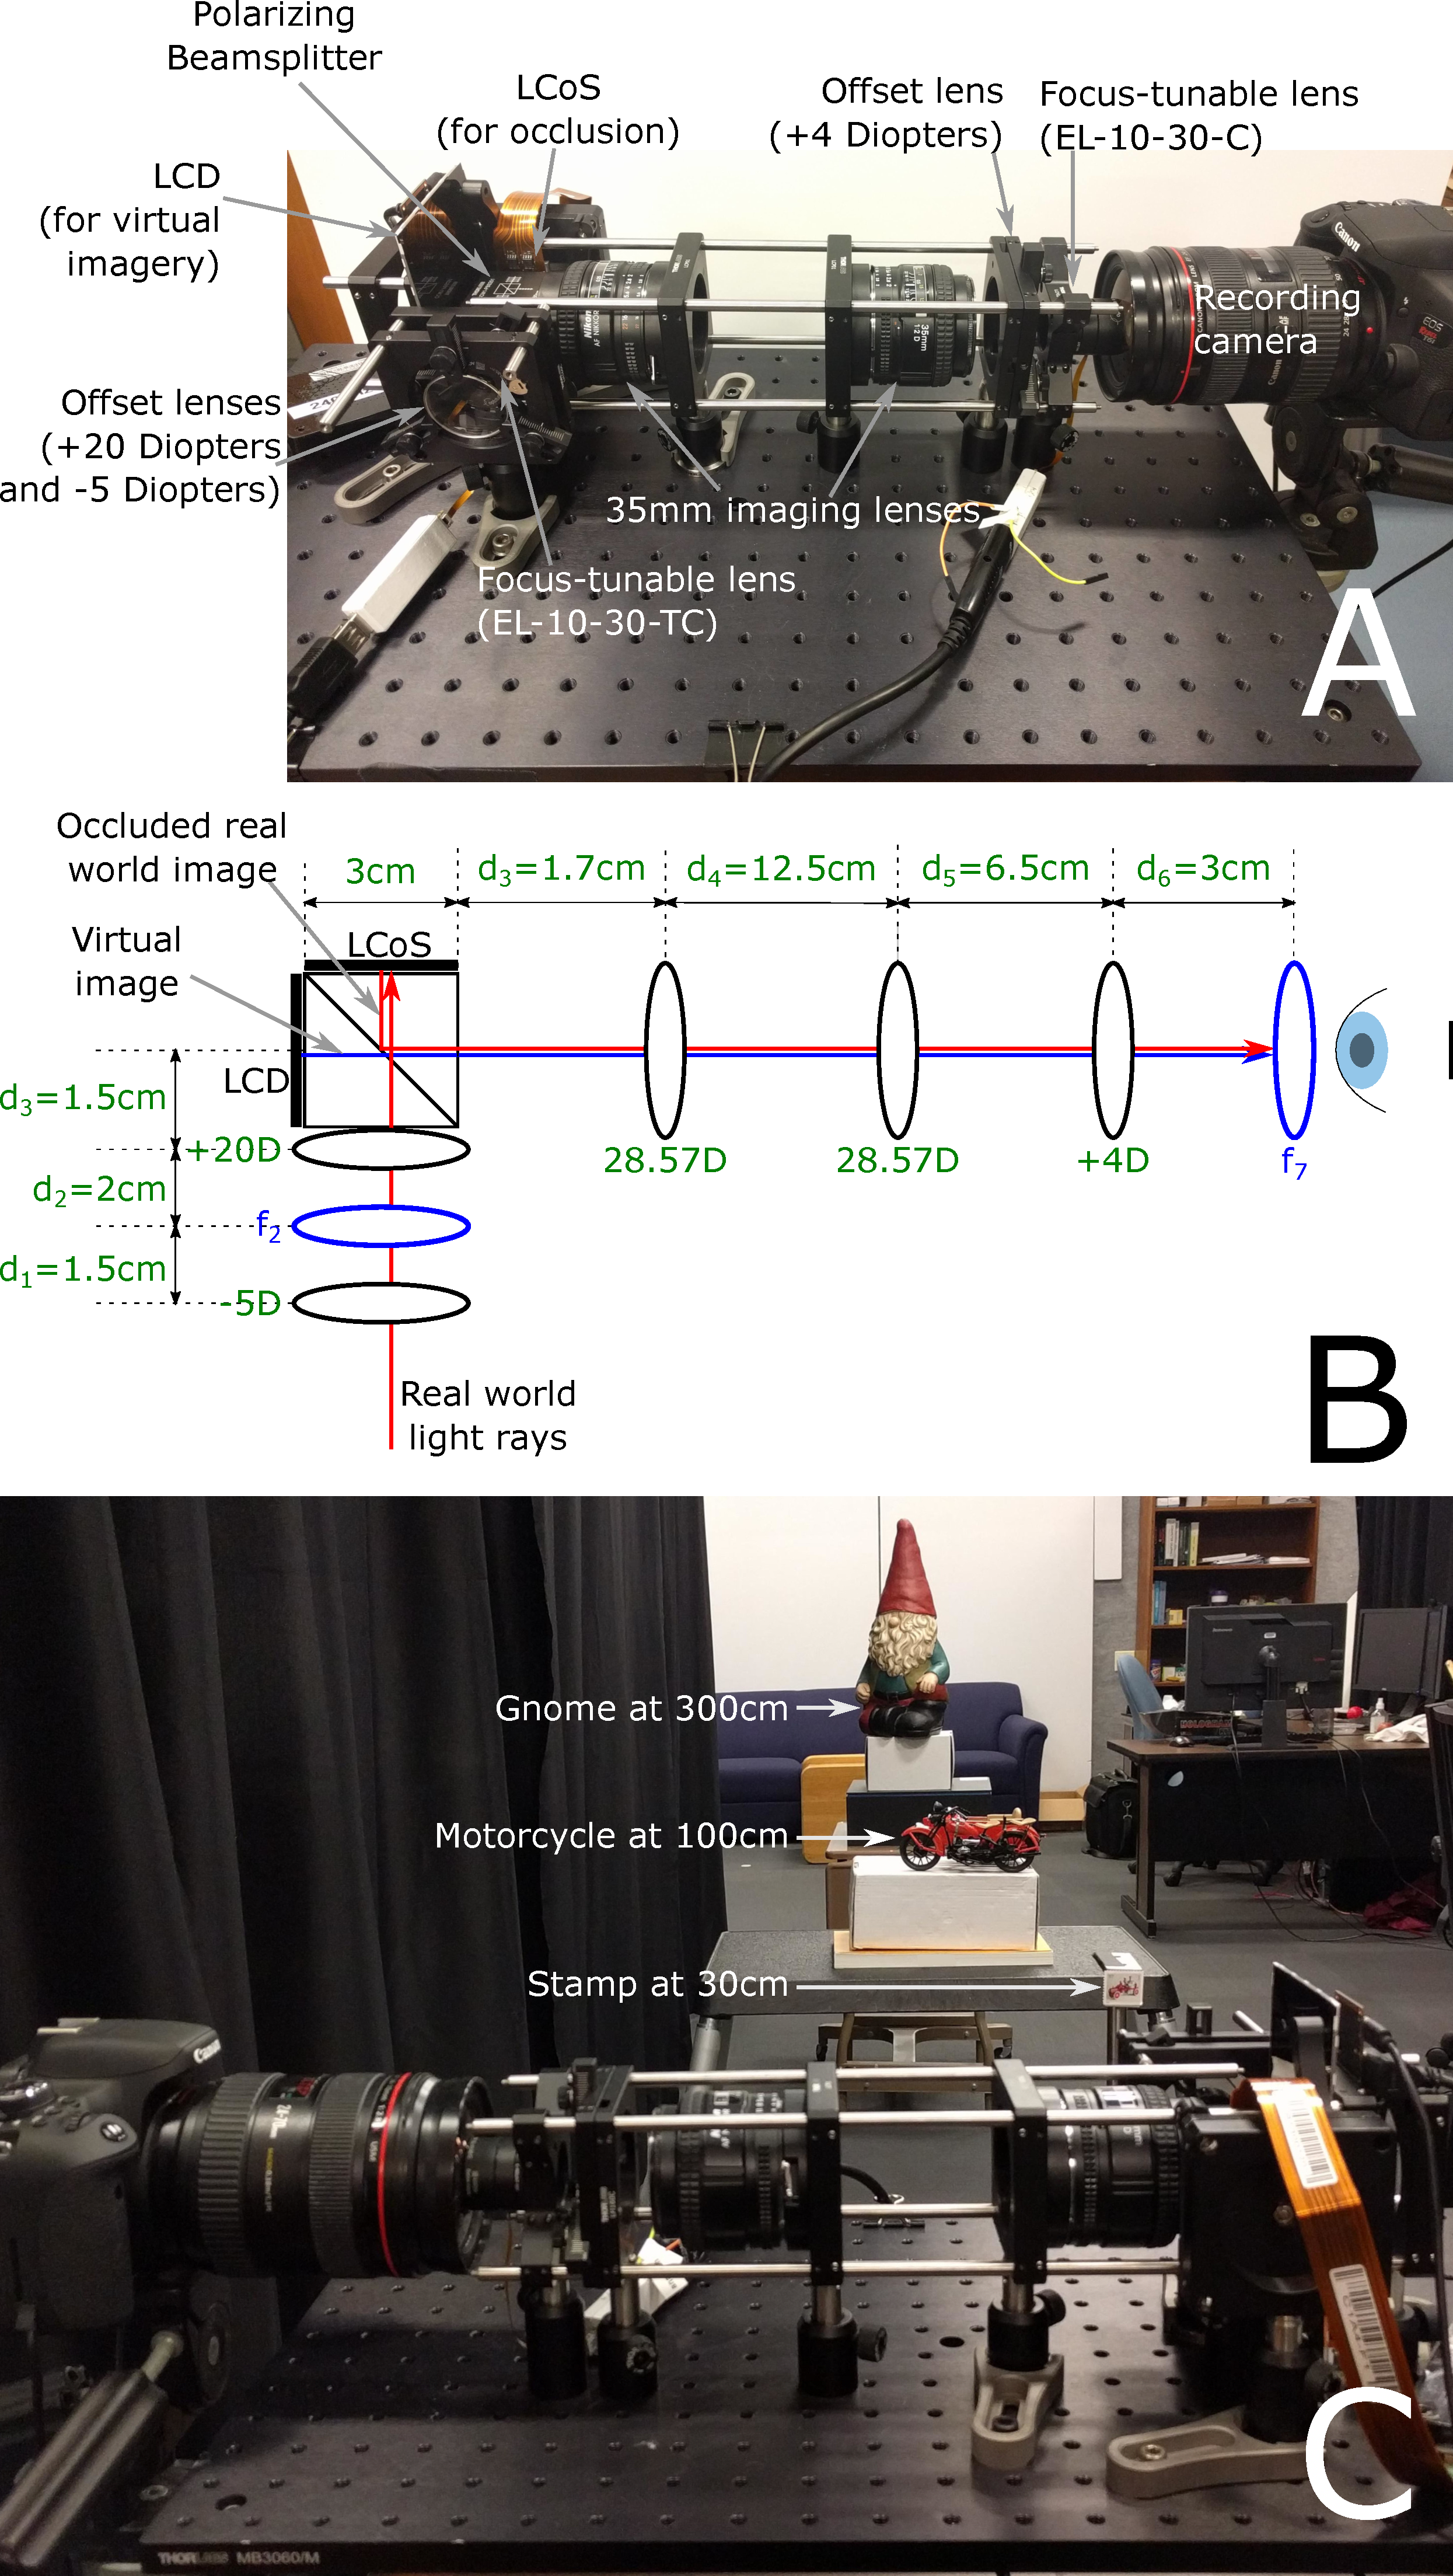
\includegraphics[width=0.46\textwidth]{images/prototype}}
\caption[Varifocal-Occlusion NED: teaser]{\textbf{Left of the vertical line:} views through our prototype AR display, which is emulating different AR display technologies for each column. 
The augmented scene is composed of real-world objects (stamp, motorcycle, and gnome) and virtual objects (ring, teapot, and bull). Objects are distributed at different depths: stamp and ring at 30cm, motorcycle and teapot at 100cm, and gnome and bull at 300cm. 
\textit{(Column 1)} Commercially available AR displays: a transparent virtual image is presented at a fixed distance. Important depth cues such as occlusion and accommodation are absent.
\textit{(Column 2)} Varifocal AR displays: virtual image can be moved to different depths, but images are still transparent. 
\textit{(Column 3)} Fixed-focus occlusion-capable AR display: 
Occlusion and virtual image is fixed at a single depth, limiting realism when the user is focused to other depths. Note how all virtual objects, including the nearby ones, are in focus when the camera is focused far, and all virtual objects are defocused when the camera is focused near. 
\textit{(Column 4)} Varifocal occlusion-capable AR displays: virtual and occlusion image plane can be moved to different depths enabling perceptually correct depth cues for occlusion and accommodation. Note how objects at the same depth, e.g., near objects (stamp and ring) or far objects (gnome and bull), are correctly in focus or defocused depending on the focus state of the user/camera.
\textbf{Right of the vertical line:} Comparison of occlusion masks between fixed-focus and varifocal occlusion-capable displays.}
\label{fig:varifocal_occlusion:teaser}
\end{figure*}
